% !TeX spellcheck = en_US 
\documentclass[report]{byu-aero}

%This sets the visible levels shown on the Table of Contents. 2 will show the Sections and Subsections. This seems okay to save some space. If you want to show subsubsections change it to 3. 1 will just show the sections, but that seems too brief.
\setcounter{tocdepth}{2}


%!!!!!!!!!!!!!!!!!!!!!!!!!!!!!!!!!!!!!!!!!!!!!!!!!!!!!!!!!!!!!!!!!!!!!!!!!!!!!!!!!!!!!!!!%
%!!!!!!! UNLESS YOU KNOW WHAT YOU'RE DOING, DO NOT TOUCH ANYTHING ABOVE THIS LINE !!!!!!!%
%!!!!!!!!!!!!!!!!!!!!!!!!!!!!!!!!!!!!!!!!!!!!!!!!!!!!!!!!!!!!!!!!!!!!!!!!!!!!!!!!!!!!!!!!%

%%%%%%%%%%%%%%%%%%%%%%%%%%%%%%%%%%
%%%%%%%%%%   Text Body   %%%%%%%%%
%%%%%%%%%%%%%%%%%%%%%%%%%%%%%%%%%%
\begin{document}

% Title Page

\includepdf[page=-]{titlepage.pdf}

%%%%%%%%%%%%%%%%%%%%%%%%%%%%%%%%%%%%%%%%%%
%%%%%%%%%%   Table of Contents   %%%%%%%%%
%%%%%%%%%%%%%%%%%%%%%%%%%%%%%%%%%%%%%%%%%%
\setcounter{page}{2} %This sets the page counter to 2, since the Title page is counted as page 1
\thispagestyle{tocpage} %This uses the alternate table of contents page header style
\tableofcontents %This makes the table of contents
%The following 3 lines add the Table of Contents "section" to the Table of Contents
%\phantomsection
%\addcontentsline{toc}{section}{Table of Contents}
%\markboth{Table of Contents}{Table of Contents}

\clearpage
\newpage

%%%%%%%%%%%%%%%%%%%%%%%%%%%%%%%%%%%%%%%%%%%%%%%%%%%%%%%%%%%%%%%%%%%%%%%%%%%%%%%%%%%%%%%%%
%%%%%%%%%%%%%%%%%%%%%%%%%%%%         EXECUTIVE SUMMARY         %%%%%%%%%%%%%%%%%%%%%%%%%%
%%%%%%%%%%%%%%%%%%%%%%%%%%%%%%%%%%%%%%%%%%%%%%%%%%%%%%%%%%%%%%%%%%%%%%%%%%%%%%%%%%%%%%%%%
\section{Executive Summary} % (5 Points)
\label{sec:ExecutiveSummary}
% Section Requirements
% 1) Maximum of 1 page. If exceeded, score as 0 points
% 2) Summary description of selected design and why it best meets the mission requirements
% 3) Main points from subsequent sections
% 4) Document the performance/capabilities of your system solution


\lipsum[1-6]

% Performance Summary Table
\begin{table}[h!]
	\centering
	\caption{Summary of major system performance factors.}
	\label{tab:performancesummary}
	\rowcolors{2}{BYUbluelite}{white}
	\begin{tabular}{ |c|c| } 
		\hline
		\rowcolor{BYUbluemid}
		Metric & \\
		\hline
		& {\color{\BYUred}[Performance (units)]} \\
		\hline
		&  {\color{\BYUred} [Performance (units)]} \\
		\hline
	\end{tabular}
\end{table}

\newpage

%%%%%%%%%%%%%%%%%%%%%%%%%%%%%%%%%%%%%%%%%%%%%%%%%%%%%%%%%%%%%%%%%%%%%%%%%%%%%%%%%%%%%%%%%
%%%%%%%%%%%%%%%%%%%%%%%%%%%%         MANAGEMENT SUMMARY        %%%%%%%%%%%%%%%%%%%%%%%%%%
%%%%%%%%%%%%%%%%%%%%%%%%%%%%%%%%%%%%%%%%%%%%%%%%%%%%%%%%%%%%%%%%%%%%%%%%%%%%%%%%%%%%%%%%%
\section{Management Summary} % (5 Points)
\label{sec:ManagementSummary}
% Section Requirements
% 1) Describe the organization of the design team
% 2) Chart of design personnel and assignments areas
% 3) Milestone chart showing planned and actual timing of major elements


%%%%%%%%%%%%%%%%%%%%%%%%%%%%%
%%% - Team Organization - %%%
%%%%%%%%%%%%%%%%%%%%%%%%%%%%%
\subsection{Team Organization}
\label{ssec:TeamOrganization}

%Team Organization Chart:
%TEAM ORGANIZATION
\begin{wrapfigure}[7]{R}{0in}
	\centering
	\raisebox{0pt}[\dimexpr\height-3\baselineskip\relax]{
\begin{tikzpicture}[node distance = 1cm, auto]

	% Place nodes
	\node [block] (Project Manager) {\footnotesize Project Manager};
%	\node [block, below left = 0.1 and -1.25cm  of Project Manager] (Engineering Lead) {\footnotesize Engineering Lead};
%	\node [block, below right = 0.1 and -1.25cm   of Project Manager] (Project Manager) {\footnotesize Project Manager};

	\node [block2, below left = 0.25 and -1.25cm of Project Manager] (Aerodynamics) {\footnotesize Aerodynamics};
	\node [block2, below left = 1.0 and -1.25cm  of Project Manager] (Structures) {\footnotesize Structures};
	\node [block2, below left = 1.75 and -1.25cm  of Project Manager] (Propulsion) {\footnotesize Propulsion};
	\node [block2, below right = 0.25 and -1.25cm  of Project Manager] (Systems) {\footnotesize Systems};
	\node [block2, below right = 1.0 and -1.25cm  of Project Manager] (Graphics) {\footnotesize Graphics};
	\node [block2, below right = 1.75 and -1.25cm  of Project Manager] (Manufacturing) {\footnotesize Manufacturing};

	% Draw edges
%	\path[line] let \p1=(Project Manager.south), \p2=(Engineering Lead.east) in (Project Manager.south) --  +(0,0.55*\y2) -| node {} (Engineering Lead.east);
%	\path[line] let \p1=(Project Manager.south), \p2=(Project Manager.west) in (Project Manager.south) -- +(0,0.55*\y2) -| node {} (Project Manager.west);

	\path[line] let \p1=(Project Manager.south), \p2=(Aerodynamics.east) in (Project Manager.south) -- +(0,0.65*\y2) -| node  {} (Aerodynamics.east);
	\path[line] let \p1=(Project Manager.south), \p2=(Systems.west) in (Project Manager.south) -- +(0,0.65*\y2) -| node  {} (Systems.west);

	\path[line] let \p1=(Project Manager.south), \p2=(Structures.east) in (Project Manager.south) -- +(0,0.8*\y2) -| node  {} (Structures.east);
	\path[line] let \p1=(Project Manager.south), \p2=(Graphics.west) in (Project Manager.south) -- +(0,0.8*\y2) -| node  {} (Graphics.west);

	\path[line] let \p1=(Project Manager.south), \p2=(Propulsion.east) in (Project Manager.south) -- +(0,0.85*\y2) -| node  {} (Propulsion.east);
	\path[line] let \p1=(Project Manager.south), \p2=(Manufacturing.west) in (Project Manager.south) -- +(0,0.85*\y2) -| node  {} (Manufacturing.west);
\end{tikzpicture}}
	\caption{Here we show the structure of, and assignment areas within, our team organization.}
	\label{fig:personnelassignments}
\end{wrapfigure} %You can change the team_organization.tex file to update this and it will automatically update in this file.


%Introduction
\Cref{fig:personnelassignments} depicts the overall organization of our team structure.  Each of the teams is lead by an individual who answers to the Engineering Lead and Project Manager.  The skills required for each position/team are as follows.

\paragraph{Engineering Lead} As with the team leads, the Engineering Lead primarily requires good decision making and leadership skills, qualities the BYU Aero Club seeks to develop in all of its members.  In addition the Engineering Lead has a well rounded understanding of the various systems and both design and testing expertise.
\paragraph{Project Manager} The Project Manager has excellent organizational skills  and oversees the logistical side of the project: heading up report writing, budgeting tasks, scheduling, etc.
\paragraph{Aerodynamics} The Aerodyanmics team members have expertise in aerodynamic analysis and testing, including skills in hand calculations, computational analysis tools, wind tunnel and glide testing.
\paragraph{Structures} The Structures team members focus on skills in structural analysis and testing, employing hand calculations, computational tools, and various structural testing methods.
\paragraph{Propulsion} The Propulsion team focuses on analyzing and testing the propulsion system effectiveness and efficiency, but also has skills in electronics related to the propulsion system.
\paragraph{Systems} The Systems team works very closely with the Engineering Lead, as they oversee all systems interfacing, avionics, etc.  There is a sub-group of the Systems team that is assigned to work on the mission specific payload and related components, as well as related testing. %TODO: consider updating this sentence to reflect the actual specialized mission requirements for the year.
\paragraph{Manufacturing} The Manufacturing team oversees the manufacturing of all prototypes and testing apparatus.
\paragraph{Graphics} The Graphics team has skills in CAD design as well as graphical marketing for the team. 


%%%%%%%%%%%%%%%%%%%%%%%%%%%%%
%%%%%%%% - Timeline - %%%%%%%
%%%%%%%%%%%%%%%%%%%%%%%%%%%%%
\subsection{Schedule}
\label{ssec:Schedule}


\begin{figure}[h!]
	\centering
%		\raisebox{0pt}[\dimexpr\height-1.5\baselineskip\relax]{
	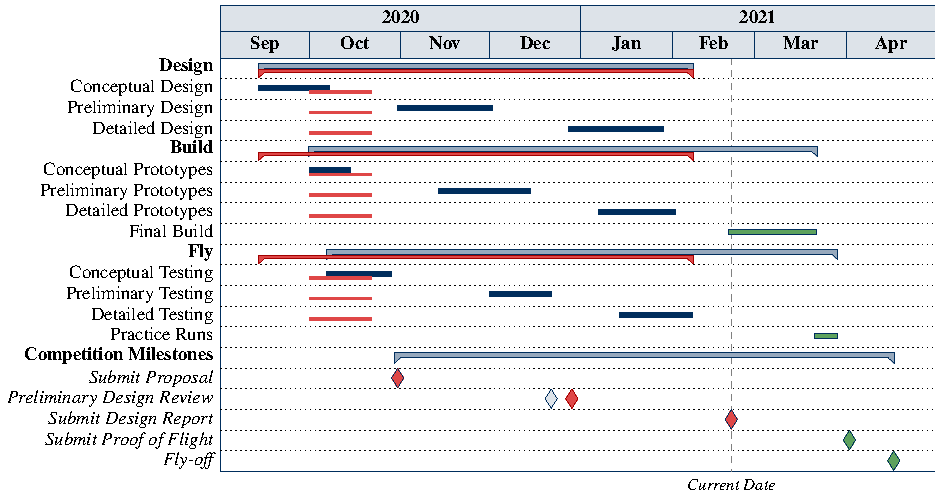
\includegraphics[]{milestonechart_dr.pdf}
%	}
	\caption{This milestone chart reveals our {\color{\BYUblue} original plan} for major elements of our design process compared to the  {\color{\BYUred} actual timing} of these events.  Note that we submitted the proposal on time, as well as this report.  We anticipate remaining on schedule for the {\color{\BYUgreen} future elements} of this chart.}
	\label{fig:plannedvsactualtiming}
\end{figure}

%timeline description.
\Cref{fig:plannedvsactualtiming} depicts our planned vs. actual timeline for the year.
 \lipsum[2]



%%%%%%%%%%%%%%%%%%%%%%%%%%%%%%%%%%%%%%%%%%%%%%%%%%%%%%%%%%%%%%%%%%%%%%%%%%%%%%%%%%%%%%%%%
%%%%%%%%%%%%%%%%%%%%%%%%%%%%         CONCEPTUAL DESIGN         %%%%%%%%%%%%%%%%%%%%%%%%%%
%%%%%%%%%%%%%%%%%%%%%%%%%%%%%%%%%%%%%%%%%%%%%%%%%%%%%%%%%%%%%%%%%%%%%%%%%%%%%%%%%%%%%%%%%
\section{Conceptual Design} % (15 Points) %Note: this should be completed already as part of the proposal
\label{sec:ConceptualDesign}
% Section Requirements
% 1) Describes mission requirements (problem statement)
% 2) Translate mission requirements into sub system design requirements
% 3) Present a scoring sensitivity analysis.
% 4) Review solution concepts/configurations considered
% 5) Describe concept weighting and selection process and results


\subsection{Mission Requirements}
\label{ssec:missionreqs}

The mission requirements for this year's competition are as follows:

\subsubsection{Airframe and Operational Constraints:}
\begin{itemize}
	\item Safety Requirements:
	\begin{itemize}
		\item {\color{\BYUred} [THIS YEAR'S REQUIREMENT(S).]}
	\end{itemize}
	\item Airframe Requirements:
	\begin{itemize}
		\item {\color{\BYUred} [THIS YEAR'S REQUIREMENT(S).]}
	\end{itemize}
	\item Payload Requirements:
	\begin{itemize}
		\item {\color{\BYUred} [THIS YEAR'S REQUIREMENT(S).]}
	\end{itemize}
	\item {\color{\BYUred} [THIS YEAR'S SPECIAL REQUIREMENT(S)]}:
	\begin{itemize}
		\item {\color{\BYUred} [THIS YEAR'S REQUIREMENT(S).]}
	\end{itemize}
\end{itemize}



\subsubsection{Flight Mission Scoring:}



\paragraph{Flight Mission 1:}



\paragraph{Flight Mission 2:}



\paragraph{Flight Mission 3:}



\subsubsection{Total Score Summary:}

\[TS = M_1 + M_2 + M_3 + GM + DR\]

where \(TS\) is total score, \(M_i\) is the score associated with the mission number subscript, \(GM\) is the ground mission score, and \(DR\) is the design report score.

\begin{figure}[h!]
	\centering
	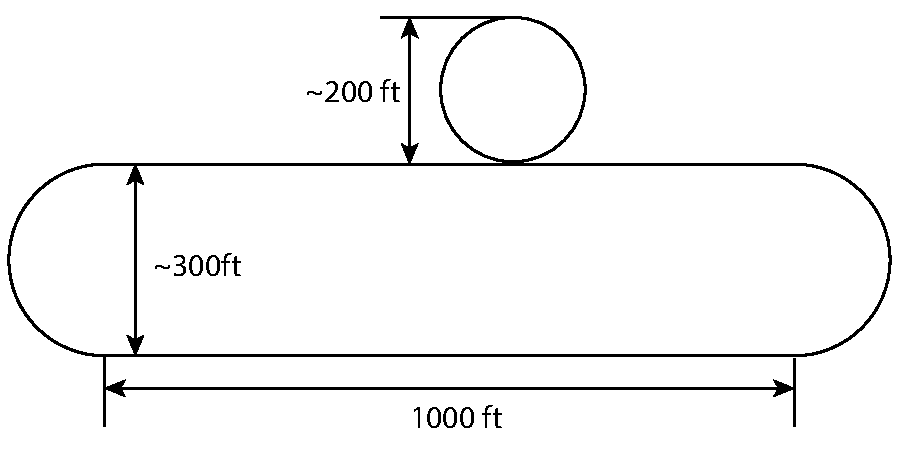
\includegraphics[width=4.5in]{coursedistances}
	\caption{This plot breaks down the estimated lengths of the course based on the scale drawing from the mission requirements.}
	\label{fig:course}
\end{figure}

%%%%%%%%%%%%%%%%%%%%%%%%%%%%%
%%%% - Sub-system Reqs - %%%%
%%%%%%%%%%%%%%%%%%%%%%%%%%%%%
\subsection{Sub-system Design Requirements}
\label{ssec:MissionReqs}

We have organized our sub-system requirements into aerodynamics, structure, propulsion, and specialty requirements explained below.

\subsubsection{Aerodynamics Requirements}
\label{sssec:AerodynamicReqs}

Some of the major requirements for the aerodynamics sub-system are: Maximize aerodynamic efficiency in order to use less energy to overcome drag for all flight missions.  Design wing loading to be able to take off and fly with design max payload weight.  Keep the wingspan within the maximum of {\color{BYUred}[MAX SPAN CONSTRAINT THIS YEAR]}.  Choose airfoil(s) and configuration that will make take off feasible in the {\color{BYUred}[THIS YEAR'S TAKE-OFF REQUIREMENT]}

\subsubsection{Structural Requirements}
\label{sssec:StructuralReqs}

The breakdown of mission requirements for the structures sub-system include: Minimize the structural weight while maintaining sufficient rigidity to keep the aerodynamics as designed, especially when full payload weight is in use.  Make sure the structure is sufficiently rigid to avoid aerodynamic flutter within the flight envelope. {\color{BYUred}[OTHER MISC. STRUCTURES REQUIREMENTS THIS YEAR (E.G. FOLDING WINGS.)]}

\subsubsection{Propulsion Requirements}
\label{sssec:PropulsionReqs}

The propulsion sub-system requirements are to: Have sufficient system efficiency and battery capacity to enable completion of the flight missions and maximizing speed with sufficient endurance while also providing sufficient thrust for {\color{BYUred}[THIS YEAR'S TAKE-OFF REQUIREMENT]}

\subsubsection{Specialty Requirements} %change this to be specifically what it is (like bomb drop or whatever the specific mission is)
\label{sssec:SpecialReqs}

{\color{BYUred}[REQUIREMENTS FOR THIS YEAR'S SPECIAL STUFF.]} 
\lipsum[2]




%%%%%%%%%%%%%%%%%%%%%%%%%%%%%%%
%%%% - Sensitivity Study - %%%%
%%%%%%%%%%%%%%%%%%%%%%%%%%%%%%%
\subsection{Scoring Sensitivity Analysis}
\label{ssec:SensitivityStudy}

%Figure related to sensitivity study, move around to get formatting correct...
\begin{figure}[h!]
	\centering
	\raisebox{0pt}[\dimexpr\height-2\baselineskip\relax]{
		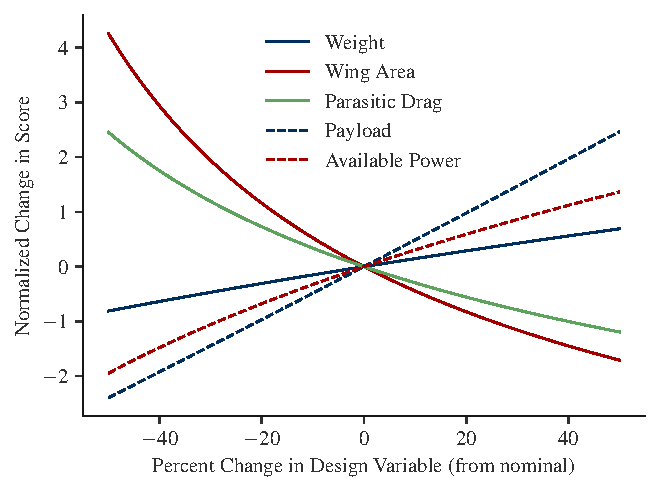
\includegraphics[]{sensitivityobj}
	}
	\caption{This plot shows the effects of those design parameters that directly affect the increase/decrease in mission scoring beyond simple completion.}
	\label{fig:sensitivity}
\end{figure}

For our sensitivity study, we first differentiated between design variables that could increase/decrease our score and those that were only related to the minimum constraints. Furthermore, some aspects of the score are insensitive by design parameters, such as the design report score, the ground mission score, and the Flight Mission 1 score.  Our total, design-sensitive score is simply the sum of scores from Flight Mission 2 and 3.

{\color{\BYUred} [BREAKDOWN OF THE MATHS USED TO PERFORM THE SENSITIVITY STUDY.]}

In order to normalize the scores as they are in the competition, we ran the analysis first without normalization, from which we saved the maximum scores like they are in competition. We then used those maxima as the normalization factors and re-ran the analysis. This way we could simulate the competition normalizations for the scoring and one mission would not dominate another unrealistically.

In our analysis (results shown in \cref{fig:sensitivity}), we found that the wing area and parasitic drag coefficient induced negative sensitivities, thus we want to minimize drag and maximize wing loading (while still being able to take off).  The available power was also important, and can be affected by increasing battery capacity, discharge rate, or voltage, or increasing propulsive efficiency. {\color{BYUred}[TAKE AWAYS FROM PAYLOAD STUFF]}. We should also note that the aircraft weight had the lowest effect on the overall sensitivity, but is incredibly important to meeting the fixed constraints of the competition.




\subsection{Concept Review, Weighting, and Selection Process}
\label{ssec:selectionprocess}

Informed by our sensitivity study, \cref{tab:fom} shows our general figures of merit for our conceptual design choices. In addition to the primary mission sensitive parameters, we added some practical figures of merit as well.  In addition, rather than having multiple figures of the same value, we chose to make each figure a distinct value, thereby requiring a true prioritization and less change of ambiguity during the selection process.

We chose weight as the most important factor because it not only relates to the mission objectives, but also concerns the take-off/landing constraints.  Drag was our next highest factor, as speed is important for maximizing flight mission scores.  We placed simplicity next, as we must be able to actually produce our chosen design with our current and realistic potential abilities.  We found stability to be important as well, since our aircraft needs to be controllable if we are to compete, but stability is relatively easy to achieve for most designs, so it was given a relatively lower value to match.  Finally {\color{\BYUred}[TALK ABOUT THE YEAR SPECIFIC METRIC IF THERE IS ONE.]} Each of the decision matrices has additional figures of merit associated with sub-system specific requirements. Note also, that parameters associated with available power were not included in the general list of figures of merit, but are included in propulsion specific decision matrices.

%----------------
%---   Figure of Merit (i.e. the weights used in decision matrices)
%----------------
\begin{table}[h!]
	\centering
	\caption{Figures of Merit}
	\label{tab:fom}
	\rowcolors{2}{BYUbluelite}{white}
	\begin{tabular}{ |c|c| } 
		\hline
		\rowcolor{BYUbluemid}
		Factor & Scale (1-5) \\
		\hline
		Weight & 10 \\
		\hline
		Drag & 8 \\
		\hline
		Simplicity & 6 \\
		\hline
		Stability & 4 \\
		\hline
		{\color{\BYUred} {\color{BYUred} [YEAR SPECIFIC ITEM]}} & 2 \\
		\hline
	\end{tabular}
\end{table}


\subsubsection{Wing Configuration Selection}

For our wing configuration, we needed to take overall potential lift into account, due to the take-off/landing requirements.  \Cref{tab:wingconfiguration} shows our scoring for single wing, tandem wing, and bi/tri-wing configurations.  Note that we eliminated flying wing/blended wing body configurations up front based on our previous experience with that concept.

\lipsum[1]


%----------------
%---   Wing Configuration Decision Matrix (Convetional, Bi-Plane, Tandem Wing, etc.)
%----------------
\begin{table}[h!]
	\centering
	\caption{Weighted decision matrix for wing configuration.}
	\label{tab:wingconfiguration}
	\rowcolors{2}{BYUbluelite}{white}
	\begin{tabular}{ |c|c|c|c|c| } 
		\hline
		\rowcolor{BYUbluemid}
    	& & Single Wing & Tandem Wing & Bi/Tri-wing \\
		\rowcolor{BYUbluemid}
		\multirow{-2}{*}{Factor} & \multirow{-2}{*}{Scale}  & \parbox[c]{1in}{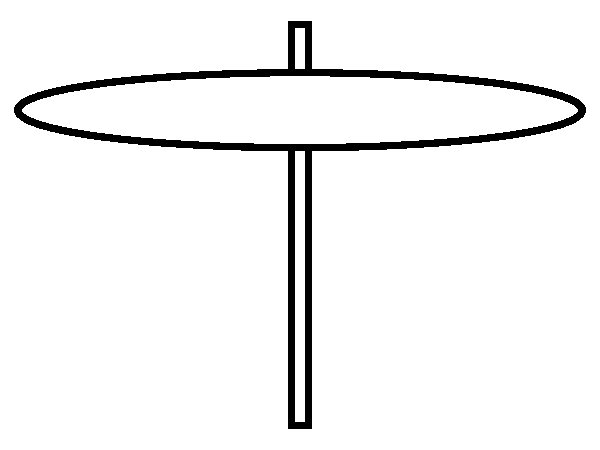
\includegraphics[width=1in]{singlewing}} & \parbox[c]{1in}{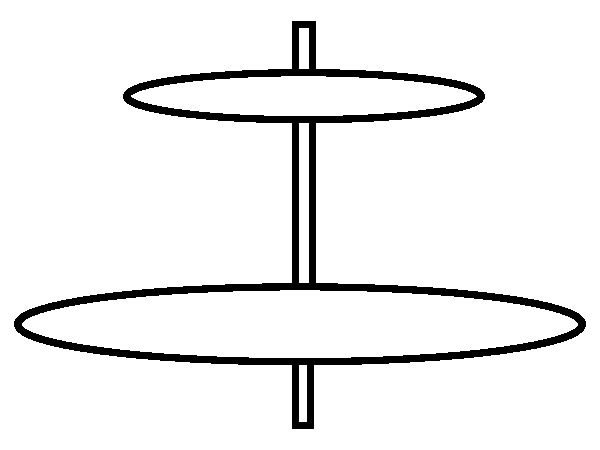
\includegraphics[width=1in]{tandemwing}} &  \parbox[c]{1in}{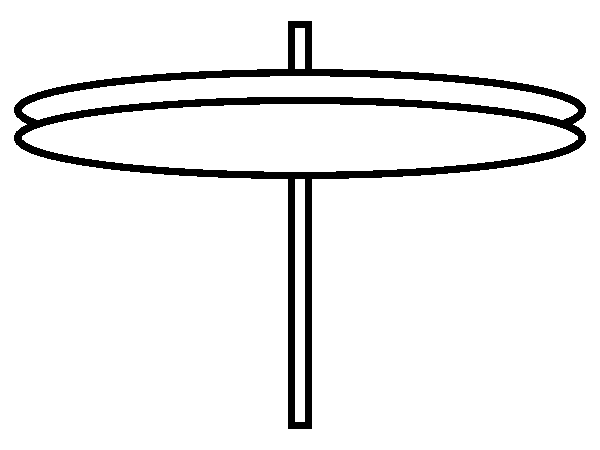
\includegraphics[width=1in]{biwing}} \\
		\hline
		Weight & 10 & 3 & 2 & 1 \\
		\hline
		Drag & 8 & 3 & 2 & 1 \\
		\hline
		Simplicity & 6 & 3 & 1 & 2 \\
		\hline
		Lift & 5 & 2 & 2 & 3 \\
		\hline
		Stability & 4 & 3 & 2 & 3 \\
		\hline
		{\color{\BYUred} {\color{BYUred} [YEAR SPECIFIC ITEM]}} & 2 & & & \\
		\hline
		\multicolumn{2}{|c|}{Totals} &  &  &  \\%BOLD WINNING OPTION
		\hline
	\end{tabular}
\end{table}

\subsubsection{Wing Placement Selection}

For the wing placement, we compared high, mid, and low wing placement.  An addition figure of merit here is the accessibility, that is, the accessibility of the payload and electronics.  This is important not only for the ground mission, but also for setting up the aircraft for flight.

\lipsum[1]


%----------------
%---   Wing Placement Decision Matrix  (High, Mid, Low)
%----------------
\begin{table}[h!]
	\centering
	\caption{Weighted decision matrix for wing placement.}
	\label{tab:wingplacement}
	\rowcolors{2}{BYUbluelite}{white}
	\begin{tabular}{ |c|c|c|c|c| } 
		\hline
		\rowcolor{BYUbluemid}
		& & High Wing & Mid Wing & Low Wing \\
		\rowcolor{BYUbluemid}
		\multirow{-2}{*}{Factor} & \multirow{-2}{*}{Scale}  & \parbox[c]{1in}{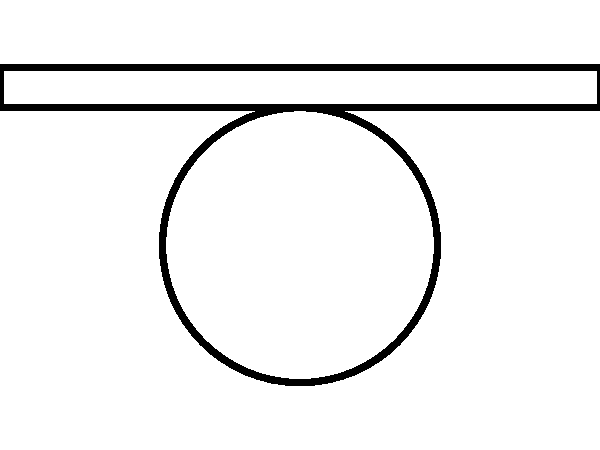
\includegraphics[width=1in]{highwing}} & \parbox[c]{1in}{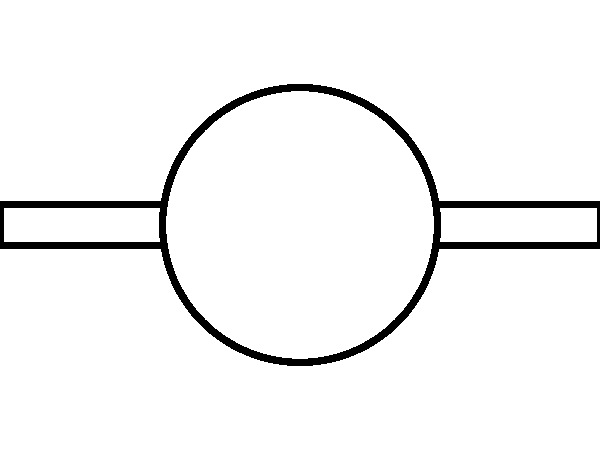
\includegraphics[width=1in]{midwing}} &  \parbox[c]{1in}{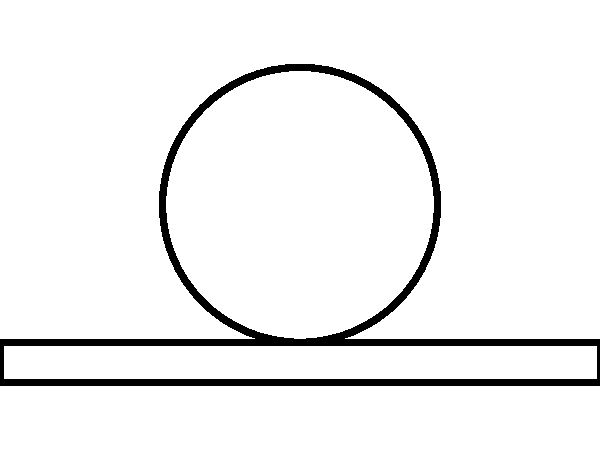
\includegraphics[width=1in]{lowwing}} \\
		\hline
		Weight & 10 & 3 & 2 & 3 \\
		\hline
		Drag & 8 & 2 & 3 & 2 \\
		\hline
		Simplicity & 6 & 3 & 1 & 2 \\
		\hline
		Accessibility & 5 & 1 & 2 & 3 \\
		\hline
		Stability & 4 & 3 & 2 & 1 \\
		\hline
		{\color{\BYUred} {\color{BYUred} [YEAR SPECIFIC ITEM]}} & 2 & & & \\
		\hline
		\multicolumn{2}{|c|}{Totals} &  &  &  \\%BOLD WINNING OPTION
		\hline
	\end{tabular}
\end{table}

\subsubsection{Empennage Configuration Selection}

For the tail configuration selection, we did not see the need for any further figures of merit.  We compared three families of configuration: T-tail family, including conventional, cruciform, and T-tail designs; V-tail family, including V- and inverted V-tail designs; and H-tail family, including U-, H-, and inverted U-tail designs.

\lipsum[1]


%----------------
%---  Tail Configuration Decision Matrix  (Conventional, H-tail, V-tail, Flying wing, etc.)
%----------------
\begin{table}[h!]
	\centering
	\caption{Weighted decision matrix for tail configuration.}
	\label{tab:tailconfiguration}
	\rowcolors{2}{BYUbluelite}{white}
	\begin{tabular}{ |c|c|c|c|c| } 
		\hline
		\rowcolor{BYUbluemid}
		& & T-Tail Variations & V-Tail Variations & H-Tail Variations \\
		\rowcolor{BYUbluemid}
		\multirow{-2}{*}{Factor} & \multirow{-2}{*}{Scale}  &
		\parbox[c]{1in}{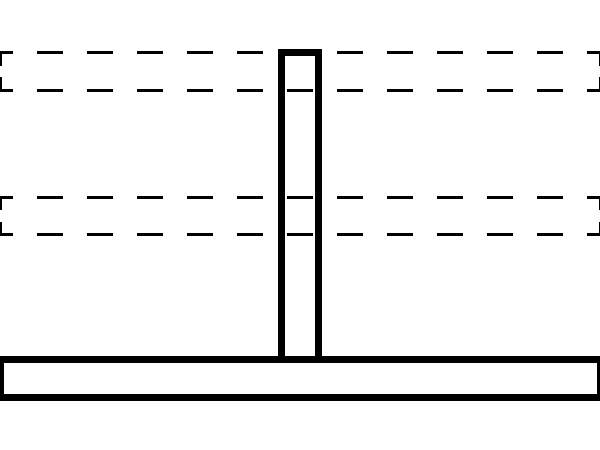
\includegraphics[width=1in]{ttail}} &
		\parbox[c]{1in}{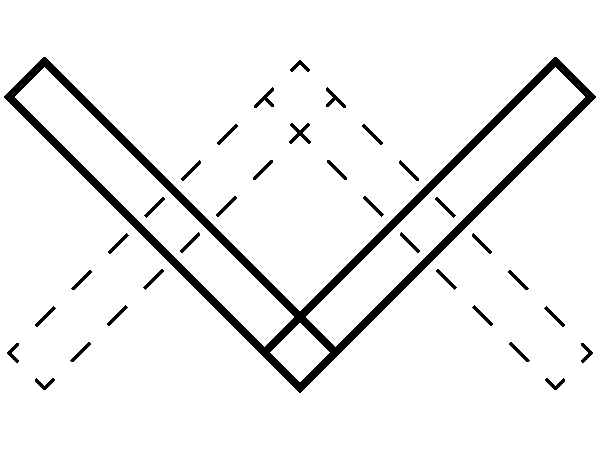
\includegraphics[width=1in]{vtail}} &
		\parbox[c]{1in}{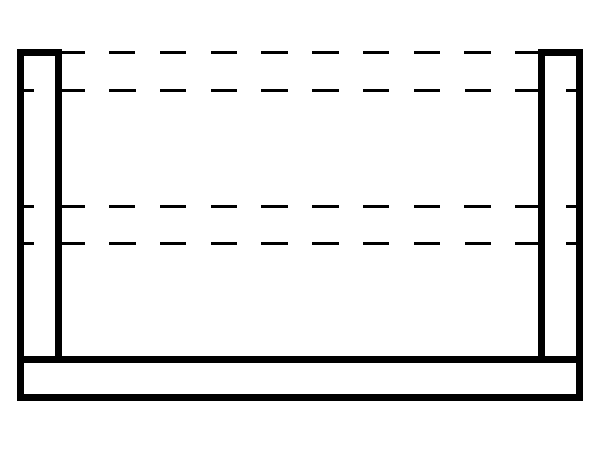
\includegraphics[width=1in]{htail}} \\
		\hline
		Weight & 10 & 2 & 3 & 1 \\
		\hline
		Drag & 8 & 2 & 3 & 2 \\
		\hline
		Simplicity & 6 & 3 & 2 & 1 \\
		\hline
		Stability & 4 & 2 & 1 & 3 \\
		\hline
		{\color{\BYUred} {\color{BYUred} [YEAR SPECIFIC ITEM]}} & 2 & & & \\
		\hline
		\multicolumn{2}{|c|}{Totals} &  &  &  \\%BOLD WINNING OPTION
		\hline
	\end{tabular}
\end{table}


\subsubsection{Propulsion Configuration Selection}

For the propulsion configuration, drag did not make sense as a figure of merit, since the system is in direct opposition to drag.  Therefore we exchanged drag for efficiency, since efficiency directly affects available power (which we found to be important in \cref{ssec:SensitivityStudy}).  We also included lift as a figure of merit for the propulsion system, because blown wing configurations can experience increased lift (due to higher induced velocities over the wing).

\lipsum[1]


%----------------
%---   Propulsion Configuration Decision Matrix  (single prop, dual prop, distributed propulsion, etc.)
%----------------
\begin{table}[h!]
	\centering
	\caption{Weighted decision matrix for propulsion configuration.}
	\label{tab:propconfiguration}
	\rowcolors{2}{BYUbluelite}{white}
	\begin{tabular}{ |c|c|c|c|c| } 
		\hline
		\rowcolor{BYUbluemid}
		& & Single Prop & Dual Prop & Distributed Prop \\
		\rowcolor{BYUbluemid}
		\multirow{-2}{*}{Factor} & \multirow{-2}{*}{Scale}  & \parbox[c]{1in}{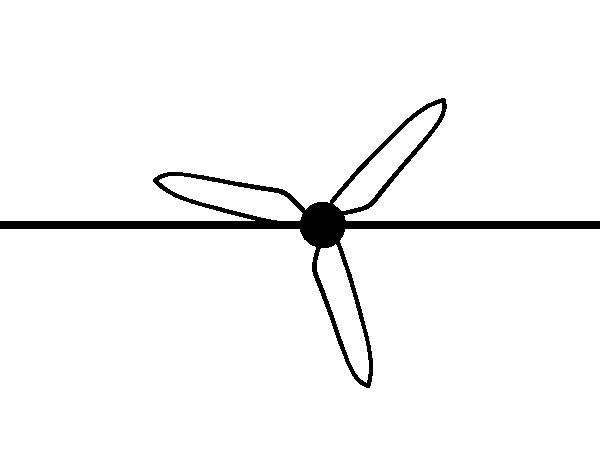
\includegraphics[width=1in]{singleprop}} & \parbox[c]{1in}{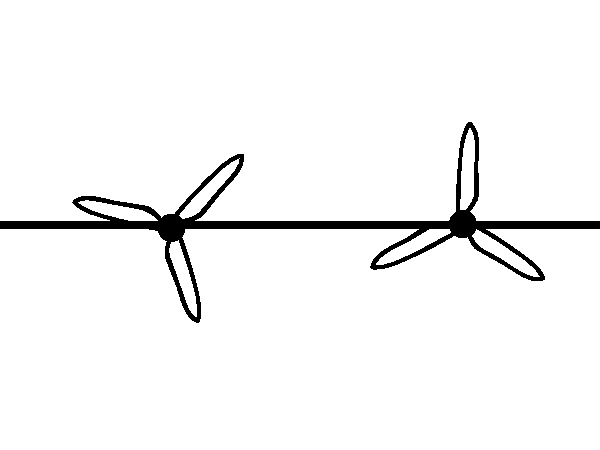
\includegraphics[width=1in]{dualprop}} &  \parbox[c]{1in}{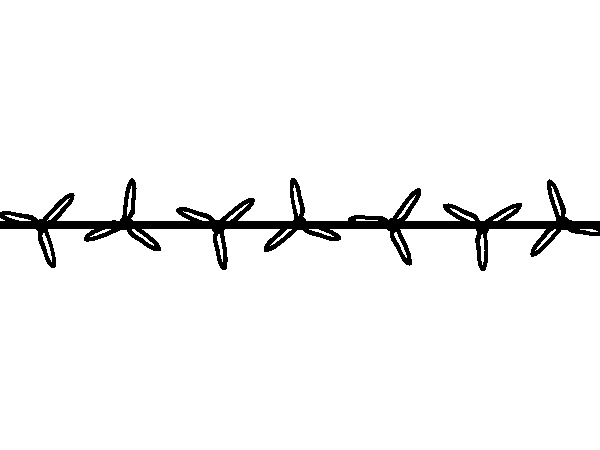
\includegraphics[width=1in]{distributedprop}} \\
		\hline
		Weight & 10 & 3 & 2 & 1 \\
		\hline
		Propulsive Efficiency & 8 & 1 & 2 & 3 \\
		\hline
		Lift & 7 & 1 & 2 & 3 \\
		\hline
		Simplicity & 6 & 3 & 2 & 1 \\
		\hline
		Stability & 4 & 3 & 2 & 3 \\
		\hline
		{\color{\BYUred} {\color{BYUred} [YEAR SPECIFIC ITEM]}} & 2 & & & \\
		\hline
		\multicolumn{2}{|c|}{Totals} &  &  &  \\%BOLD WINNING OPTION
		\hline
	\end{tabular}
\end{table}

\subsubsection{Propulsion Placement Selection}



\lipsum[1]


%----------------
%---   Propulsion Placement Decision Matrix  (tractor, pusher, etc)
%----------------
\begin{table}[h!]
	\centering
	\caption{Weighted decision matrix for propulsion placement.}
	\label{tab:propplacement}
	\rowcolors{2}{BYUbluelite}{white}
	\begin{tabular}{ |c|c|c|c|c| } 
		\hline
		\rowcolor{BYUbluemid}
		& & Pull Variations & Push Variations & Combinations \\
		\rowcolor{BYUbluemid}
		\multirow{-2}{*}{Factor} & \multirow{-2}{*}{Scale}  & 
		\parbox[c]{1in}{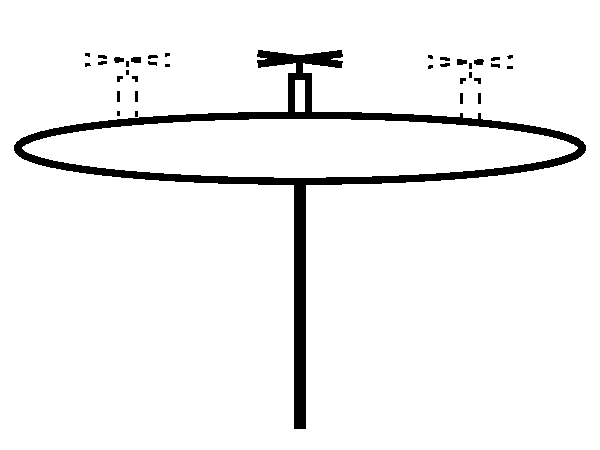
\includegraphics[width=1in]{puller}} &
		\parbox[c]{1in}{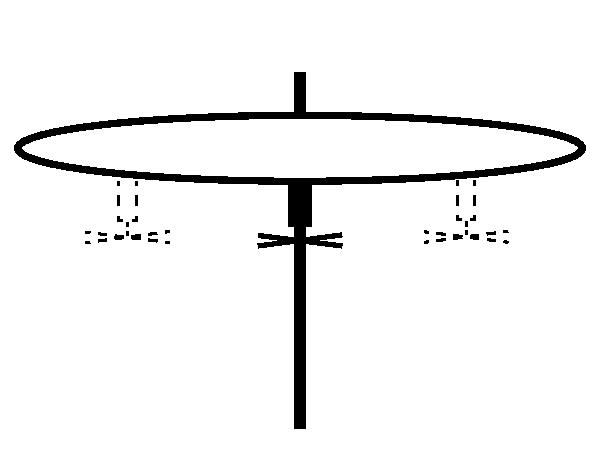
\includegraphics[width=1in]{pusher}} &
		\parbox[c]{1in}{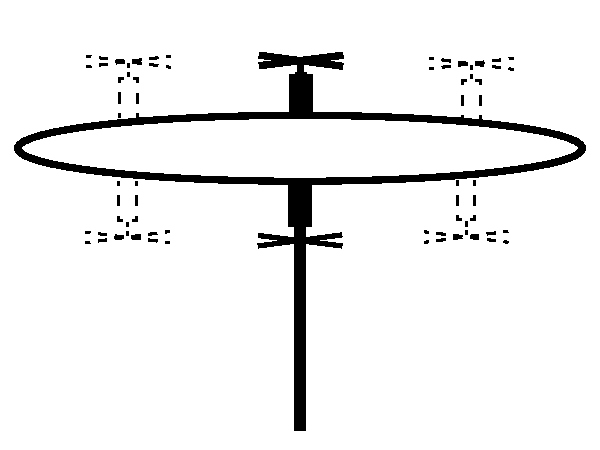
\includegraphics[width=1in]{combopushpull}} \\
		\hline
		Weight & 10 & 3 & 3 & 3 \\
		\hline
		Lift & 4 & 3 & 1 & 2 \\
		\hline
		Simplicity & 6 & 3 & 2 & 1 \\
		\hline
		Propulsive Efficiency & 4 & 3 & 1 & 2 \\
		\hline
		{\color{\BYUred} {\color{BYUred} [YEAR SPECIFIC ITEM]}} & 2 & & & \\
		\hline
		\multicolumn{2}{|c|}{Totals} &  &  &  \\%BOLD WINNING OPTION
		\hline
	\end{tabular}
\end{table}

\subsubsection{Payload}
\label{sssec:payloadconcept}

\lipsum[1]


%----------------
%---   Payload Decision Matrix.
%----------------
\begin{table}[h!]
	\centering
	\caption{Weighted decision matrix for {\color{\BYUred} [SPECIFY THIS YEAR'S PAYLOAD DESIGN]}.}
	\label{tab:payloadconfiguration}
	\rowcolors{2}{BYUbluelite}{white}
	\begin{tabular}{ |c|c|c|c|c| } 
		\hline
		\rowcolor{BYUbluemid}
		& & {\color{BYUred} [OPTION]} & {\color{BYUred} [OPTION]} & {\color{BYUred} [OPTION]} \\
		\rowcolor{BYUbluemid}
		\multirow{-2}{*}{Factor} & \multirow{-2}{*}{Scale}  & \parbox[c]{1in}{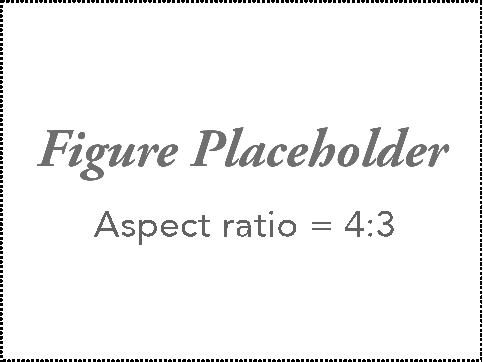
\includegraphics[width=1in]{draft4x3}} & \parbox[c]{1in}{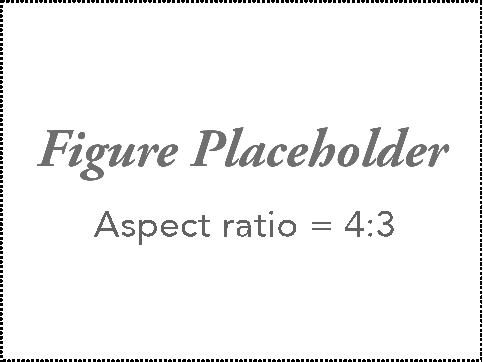
\includegraphics[width=1in]{draft4x3}} &  \parbox[c]{1in}{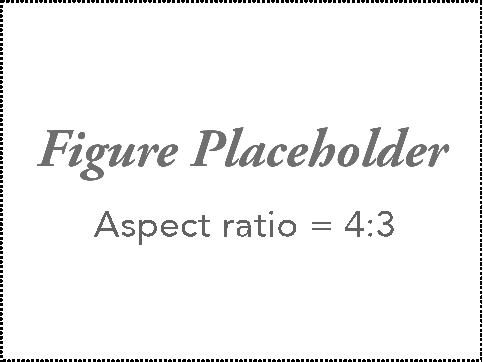
\includegraphics[width=1in]{draft4x3}} \\
		\hline
		Weight & 10 & & &\\
		\hline
		Strength & 8 & & & \\
		\hline
		Simplicity & 6 & & & \\
		\hline
		Durability & 4 & & & \\
		\hline
		{\color{\BYUred} {\color{BYUred} [YEAR SPECIFIC ITEM]}} & 2 & & & \\
		\hline
		\multicolumn{2}{|c|}{Totals} &  &  &  \\%BOLD WINNING OPTION
		\hline
	\end{tabular}
\end{table}


\lipsum[1]


\subsubsection{Final Concept}
\label{sssec:finalconcept}

\lipsum[1]

%----------------
%---  Figure of the final concept
%----------------
\begin{figure}[h!]
	\centering
	\begin{subfigure}[b]{0.475\textwidth}
		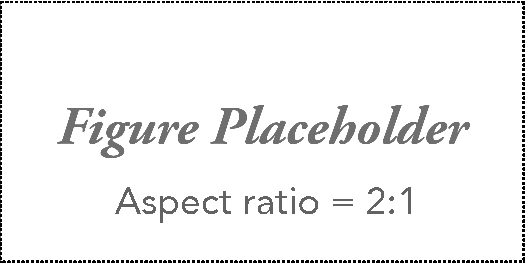
\includegraphics[width=\textwidth]{draft2x1}
		\caption{Top View}
		\label{fig:topview}
	\end{subfigure}
	%
	\begin{subfigure}[b]{0.475\textwidth}
		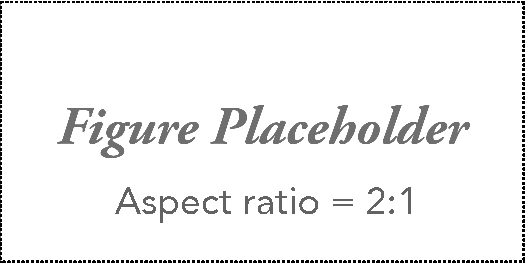
\includegraphics[width=\textwidth]{draft2x1}
		\caption{Side View}
		\label{fig:sideview}
	\end{subfigure}
	
	\begin{subfigure}[b]{0.475\textwidth}
		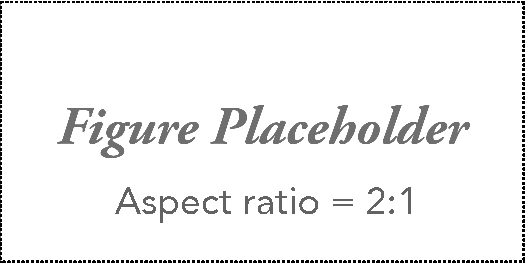
\includegraphics[width=\textwidth]{draft2x1}
		\caption{Front View}
		\label{fig:frontview}
	\end{subfigure}
	%
	\begin{subfigure}[b]{0.475\textwidth}
		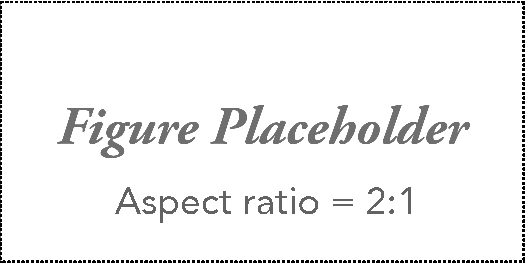
\includegraphics[width=\textwidth]{draft2x1}
		\caption{Rendered View}
		\label{fig:renderedview}
	\end{subfigure}
	\caption{Drawings and rendering of our conceptual aircraft design.}
	\label{fig:prelimdrawings}
\end{figure}



%%%%%%%%%%%%%%%%%%%%%%%%%%%%%%%%%%%%%%%%%%%%%%%%%%%%%%%%%%%%%%%%%%%%%%%%%%%%%%%%%%%%%%%%%
%%%%%%%%%%%%%%%%%%%%%%%%%%%%         PRELIMINARY DESIGN        %%%%%%%%%%%%%%%%%%%%%%%%%%
%%%%%%%%%%%%%%%%%%%%%%%%%%%%%%%%%%%%%%%%%%%%%%%%%%%%%%%%%%%%%%%%%%%%%%%%%%%%%%%%%%%%%%%%%
\section{Preliminary Design} % (20 Points)
\label{sec:PreliminaryDesign}
% Section Requirements
% 1) Describe design/analysis methodology
% 2) Document design/sizing trades
% 3) Describe/document methodology for prediction of aircraft performance (include capabilities and uncertainties)
% 4) Provide estimates of the aircraft lift, drag and stability characteristics and method of prediction
% 5) Provide estimates of the aircraft mission performance 


\subsection{Methodology}
\label{ssec:methodology}

\subsubsection{Quantify Basic Constraints}
\label{sssec:constraints}

The sensitivity study presented in \cref{ssec:SensitivityStudy} did not include any constraints, but rather simple sensitivities that informed our conceptual design choices.  To begin a preliminary design, we first needed to translate the given constraints (listed in \cref{ssec:MissionReqs}) into mathematical formulas for rapid comparison and trade studies. Aside from the obvious constraints (such as the wing span constraint), we determined the following to be important expressions.

\paragraph{Stall Speed}

\[V_\text{stall} = \left[ \frac{2W}{\rho S_\text{ref} C_{L_\text{max}}} \right]^{1/2}\]

Where \(V_\text{stall}\) is the stall speed, \(W\) is the total aircraft weight, \(\rho\) is the ambient air density, \(S_\text{ref}\) is the reference wing area, and \(C_{L_\text{max}}\) is the maximum aircraft lift coefficient.

\paragraph{Take-off Distance}

\[ d_{LO} = \frac{ W^{5/2} }{ \left( \rho S_\text{ref} C_{L_\text{max}} \right)^{3/2} P_\text{net} } \]
Where \(d_{LO}\) is the distance to lift-off, \(P_\text{net}\) is the net power, that is, the power accounting for both thrust and drag, and the other variables are as defined previously.

\paragraph{Maximum Speed}

\[ V_\text{max} = \left[ \frac{ \frac{T_a}{S_\text{ref}} + \frac{W}{S_\text{ref}}\sqrt{\left(\frac{T_a}{W}\right)^2 - 4C_{D_0}K } }{\rho C_{D_0}} \right]^{1/2} \]

Where \(V_\text{max}\) is the maximum velocity, \(T_a\) is the available thrust, \(C_{D_0}\) is the zero-lift drag coefficient of the aircraft, and \(K\) is an empirical constant assumed here to be 0.38.

\paragraph{Maximum Range}

\[R = \frac{e_b}{g} \eta \frac{L}{D} \frac{m_b}{m_\text{tot}}\]

Where \(R\) is the total range; \(e_b\) is the battery energy per unit mass; \(g\) is the gravitational constant; \(\eta\) is the combination of efficiency factors from the battery, motor, and propeller (\(\eta=\eta_b\eta_m\eta_p\)); \(L/D\) is the aircraft lift to drag ratio, and \(m_b/m_\text{tot}\) is ratio of the battery mass to total aircraft mass.

\paragraph{\(C_L\) for Maximum Efficiency (and Range)}

\[C_{L_\text{max L/D}} = \left[ C_{D_p} \pi S_\text{ref} Re \right]^{1/2}\]

Where \(C_{D_p}\) is the parasitic drag coefficient for the aircraft, \(Re\) is the Reynolds number, and other variables are defined previously.


\paragraph{Climb Rate}

\[ v_z = \frac{V_\infty \left(T - D\right)}{W}\]

Where \(v_z\) is the vertical climb rate, \(V_\infty\) is the flight velocity of the aircraft, \(T\) is the thrust force magnitude, and \(D\) is the drag force magnitude.


\paragraph{Coordinated Turn Radius}

\[r_\text{turn} = \frac{V^2}{g \tan\phi}\]

Where \(r_\text{turn}\) is the turn radius, \(V\) is the aircraft speed, and \(\phi\) is the bank angle of the aircraft.

\paragraph{Coordinated Turn Load Factor}

\[n = \frac{1}{\cos\phi}\]

Where \(n\) is the load factor.

\subsubsection{Analysis Models}


\paragraph{Weight Estimation}


\paragraph{Propulsion Model}


\paragraph{Vortex Lattice Method (XFLR5, AVL, or VLM.jl)}


\paragraph{Structures Stuff (Beams, composites, etc.)}


\paragraph{Code}




\subsection{Trade Studies}
\label{ssec:tradestudies}

\begin{equation}
	\label{eqn:optdef}
	\begin{aligned}
		\text{maximize}: 
		& ~~M2 + M3 \\
		\text{with respect to}:
		& ~~W, S_\text{ref}, C_{D_0}, \text{\color{\BYUred} [PAYLOAD STUFF]}, P_a \\
		\text{subject to}: 
		& ~~V_\text{stall}, V_\text{maneuver}, d_{LO}, R, r_\text{turn}
	\end{aligned}
\end{equation}

where \(V_\text{maneuver}\) is the maximum velocity boundary associated with structural failure due to maneuver acceleration.


\subsubsection{Wing Design}

\paragraph{Airfoil(s)}

\subsubsection{Wing/Tail Design}

\subsubsection{Fuselage}

\subsubsection{Payload}

\subsubsection{\color{\BYUred} [DESIGN TRADE STUDIES TO FIND THE ANSWER TO THE OPTIMIZATION PROBLEM.]}


\subsection{Estimated Aircraft Performance}
\label{ssec:estaircraftperfomance}

\subsubsection{Performance Prediction Methodologies and Uncertainties}
\label{sssec:uncertaintyanalysis}




\subsubsection{Lift and Drag}
\label{sssec:liftdrag}




\subsubsection{Stability}
\label{sssec:stability}



\subsubsection{Mission Performance}
\label{sssec:missionperformance}


%----------------
%---  V-n Diagram
%----------------
\begin{figure}[h!]
	\centering
	
\includegraphics[width=5in]{draft.pdf}
	\caption{V-n diagram for our preliminary aircraft design.}
	\label{fig:vndiagram}
\end{figure}



%%%%%%%%%%%%%%%%%%%%%%%%%%%%%%%%%%%%%%%%%%%%%%%%%%%%%%%%%%%%%%%%%%%%%%%%%%%%%%%%%%%%%%%%%
%%%%%%%%%%%%%%%%%%%%%%%%%%%%           DETAIL DESIGN           %%%%%%%%%%%%%%%%%%%%%%%%%%
%%%%%%%%%%%%%%%%%%%%%%%%%%%%%%%%%%%%%%%%%%%%%%%%%%%%%%%%%%%%%%%%%%%%%%%%%%%%%%%%%%%%%%%%%
\section{Detail Design} % (15 Points + 15 Points for Drawing Package)
\label{sec:detaildesign}
% Section Requirements
% 1) Document dimensional parameters of final design
% 2) Document structural characteristics/capabilities of final design
% 3) Document systems and sub-systems selection/integration/architecture
% 4) Document Weight and Balance for final design
% 5) Must include Weight \& Balance table empty and with each possible payload/configuration
% 6) Document flight performance parameters for final design
% 7) Document mission performance for final design




\subsection{Sizing}
\label{ssec:sizing}




\subsection{Structures}
\label{ssec:structures}




\subsection{Systems and Sub-system Selection, Integration, and Architecture}
\label{ssec:systemdetails}




\subsection{Weights and Balance}
\label{ssec:weightsandbalance}


%----------------
%---  Weight and Balance Table
%----------------
\begin{table}[h!]
	\centering
	\caption{Weight and Balance table including empty aircraft and each possible configuration.}
	\label{tab:wieghtsandbalance}
	\rowcolors{2}{BYUbluelite}{white}
	\begin{tabular}{ |c|c|c| } 
		\hline
		\rowcolor{BYUbluemid}
    	Configuration & Weight (grams) & CG Location (mm) \\
		\hline
	    Mission 1 (Empty) &  &  \\
		\hline
		Mission 2 &  &  \\
		\hline
		Mission 3 &  &  \\
		\hline
	\end{tabular}
\end{table}



\subsection{Expected Flight Performance Parameters}
\label{ssec:flightperformanceparams}




\subsection{Expected Mission Performance}
\label{ssec:missionperformance}



 
\subsection{Drawing Package}
\label{ssec:drawings}

The following are drawings including a 3-View drawing with dimensions of all configurations, a structural arrangement drawing, a systems layout/location drawing, and payload accommodation drawings.

%%%%%%%%%%%%%%%%%%%%%%%%%%%%%%%%%%%%%%%%%%%%%%
%%%%%%%%%%%%%   DRAWING PACKAGE   %%%%%%%%%%%%
%%%%%%%%%%%%%%%%%%%%%%%%%%%%%%%%%%%%%%%%%%%%%%
% Drawing package Requirements:
% 1) 3-View drawing with dimensions of all configurations
% 2) Structural arrangement drawing
% 3) Systems layout/location drawing
% 4) Payload(s) accommodation drawing(s)


%----------------
% 3-view drawing

\includepdf[page=-]{draft.pdf}
%----------------
% Structural Arrangement Drawing

\includepdf[page=-]{draft.pdf}
%----------------
% Systems Layout/Location Drawing

\includepdf[page=-]{draft.pdf}
%----------------
% Payload Accommodation drawing

\includepdf[page=-]{draft.pdf}
%----------------


%%%%%%%%%%%%%%%%%%%%%%%%%%%%%%%%%%%%%%%%%%%%%%%%%%%%%%%%%%%%%%%%%%%%%%%%%%%%%%%%%%%%%%%%%
%%%%%%%%%%%%%%%%%%%%%%%%%%          MANUFACTURING PLAN          %%%%%%%%%%%%%%%%%%%%%%%%%
%%%%%%%%%%%%%%%%%%%%%%%%%%%%%%%%%%%%%%%%%%%%%%%%%%%%%%%%%%%%%%%%%%%%%%%%%%%%%%%%%%%%%%%%%
\section{Manufacturing Plan} % (5 Points)
\label{sec:ManufacturingPlan}
% Section Requirements
% 1) Document the process selected for major component manufacture
% 2) Manufacturing processes investigated and selection process and results
% 3) Manufacturing milestones chart: plan and actual

\Cref{tab:fomman} shows our figures of merit for our manufacturing technique decision matrices.  Note that we prioritized in a similar fashion to our design figures with some changes to more applicable figures.  First, again, is weight.  The lower the aircraft weight, the more points can be had through {\color{\BYUred} {\color{BYUred} [YEAR SPECIFIC ITEM]}}.  After weight, we prioritized strength, as our structures need to be able to carry the loads required.  Third is simplicity; we need to be able to actually manufacture something with a given technique.  Note that simplicity is relative to our team's expertise at the time of our decisions and feasible future abilities within the time frame of the competition.  We next chose to include durability.  It is not very high on our list since we would hope to be able to design an aircraft that has no unscheduled landings, however, one cannot predict the future enough to know whether or not durability will be required, and experience shows that it most likely will.  Finally, {\color{\BYUred}[TALK ABOUT THE YEAR SPECIFIC METRIC IF THERE IS ONE.]} Because many of these factors depend on intelligent design (e.g. a built-up balsa wing could be heavier than a foam core wing, depending on how it is designed), as well as manufacturer skill, we did some prototyping and testing of representative models before completing our decision factor calculations.


%----------------
%---  Figure of Merit (i.e. the weights used in decision matrices)
%----------------
\begin{table}[h!]
	\centering
	\caption{Figures of Merit}
	\label{tab:fomman}
	\rowcolors{2}{BYUbluelite}{white}
	\begin{tabular}{ |c|c| } 
		\hline
		\rowcolor{BYUbluemid}
		Factor & Relative Importance (1-5) \\
		\hline
		Weight & 10 \\
		\hline
		Strength & 8 \\
		\hline
		Simplicity & 6 \\
		\hline
		Durability & 4 \\
		\hline
		{\color{\BYUred} {\color{BYUred} [YEAR SPECIFIC ITEM]}} & 2 \\
		\hline
	\end{tabular}
\end{table}


%----------------
%---   Wing Manufacture Decision Matrix  (single prop, dual prop, distributed propulsion, etc.)
%----------------
\begin{table}[h!]
	\centering
	\caption{Weighted decision matrix for wing manufacturing technique. Factors here come from our initial testing of balsa and fiber reinforced polymer (FRP) techniques.}
	\label{tab:wingmanufacturedecision}
	\rowcolors{2}{BYUbluelite}{white}
	\begin{tabular}{ |c|c|c|c|c| } 
		\hline
		\rowcolor{BYUbluemid}
		& & Foam Core FRP & Hollow Core FRP & Built-up/Balsa \\
		\rowcolor{BYUbluemid}
		\multirow{-2}{*}{Factor} & \multirow{-2}{*}{Scale}  &
		\parbox[c]{1in}{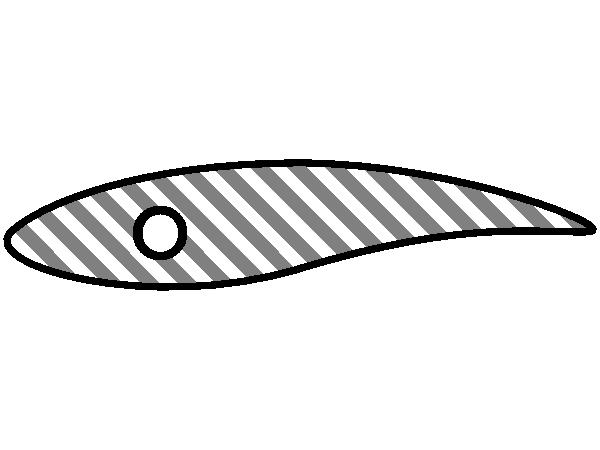
\includegraphics[width=1in]{foamcore}} & \parbox[c]{1in}{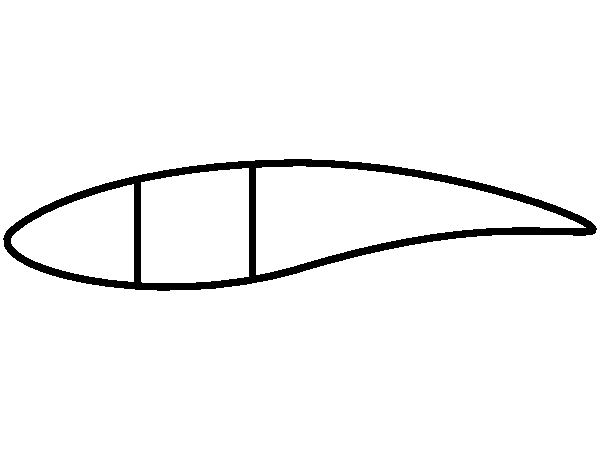
\includegraphics[width=1in]{hollowcore}} &  \parbox[c]{1in}{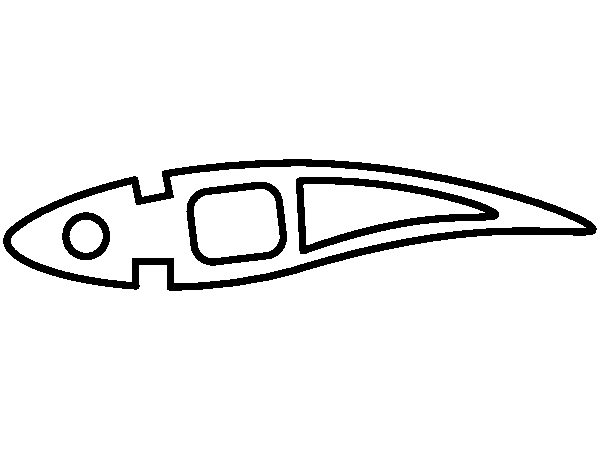
\includegraphics[width=1in]{balsa}} \\
		\hline
		Weight & 10 & & & \\
		\hline
		Strength & 8 & & & \\
		\hline
		Simplicity & 6 & & & \\
		\hline
		Durability & 4 & & & \\
		\hline
		{\color{\BYUred} {\color{BYUred} [YEAR SPECIFIC ITEM]}} & 2 & & & \\
		\hline
		\multicolumn{2}{|c|}{Totals} &  &  &  \\%BOLD WINNING OPTION
		\hline
	\end{tabular}
\end{table}


%----------------
%---   Tail Manufacture Decision Matrix  (single prop, dual prop, distributed propulsion, etc.)
%----------------
\begin{table}[h!]
	\centering
	\caption{Weighted decision matrix for tail manufacturing technique.}
	\label{tab:tailmanufacturedecision}
	\rowcolors{2}{BYUbluelite}{white}
\begin{tabular}{ |c|c|c|c|c| } 
	\hline
	\rowcolor{BYUbluemid}
	& & Foam Core FRP & Hollow Core FRP & Built-up/Balsa \\
	\rowcolor{BYUbluemid}
	\multirow{-2}{*}{Factor} & \multirow{-2}{*}{Scale}  &
	\parbox[c]{1in}{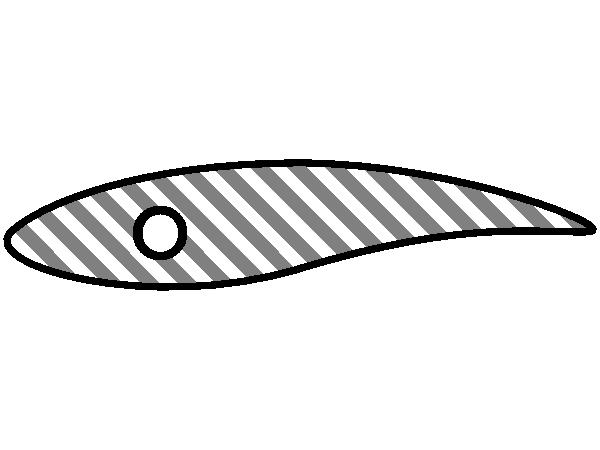
\includegraphics[width=1in]{foamcore}} & \parbox[c]{1in}{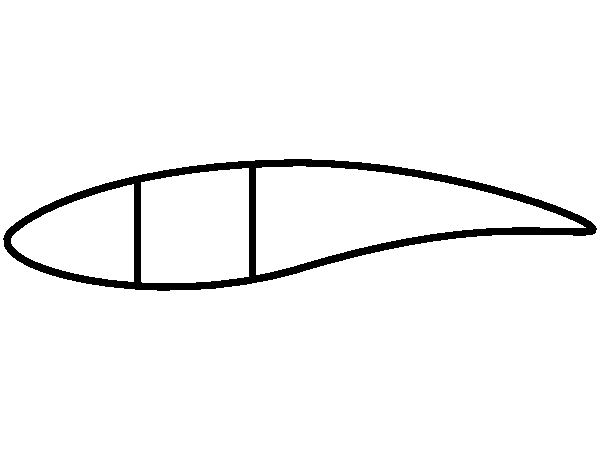
\includegraphics[width=1in]{hollowcore}} &  \parbox[c]{1in}{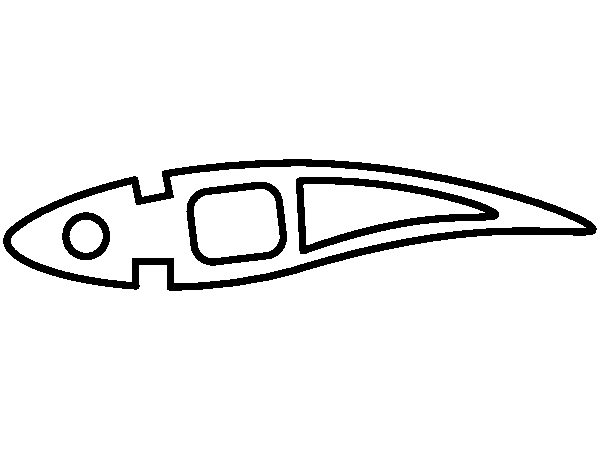
\includegraphics[width=1in]{balsa}} \\
	\hline
	Weight & 10 & & & \\
	\hline
	Strength & 8 & & & \\
	\hline
	Simplicity & 6 & & & \\
	\hline
	Durability & 4 & & & \\
	\hline
	{\color{\BYUred} {\color{BYUred} [YEAR SPECIFIC ITEM]}} & 2 & & & \\
	\hline
	\multicolumn{2}{|c|}{Totals} &  &  &  \\%BOLD WINNING OPTION
	\hline
\end{tabular}
\end{table}



%----------------
%---   Fuselage Manufacture Decision Matrix  (single prop, dual prop, distributed propulsion, etc.)
%----------------
\begin{table}[h!]
	\centering
	\caption{Weighted decision matrix for fuselage manufacturing technique.}
	\label{tab:fuselagemanufacturingdecision}
	\rowcolors{2}{BYUbluelite}{white}
	\begin{tabular}{ |c|c|c|c|c| } 
		\hline
		\rowcolor{BYUbluemid}
		& & 3D Printing & Hollow Core FRP & Built-up/Balsa \\
		\rowcolor{BYUbluemid}
		\multirow{-2}{*}{Factor} & \multirow{-2}{*}{Scale}  & \parbox[c]{1in}{
\includegraphics[width=1in]{3dprint}} & \parbox[c]{1in}{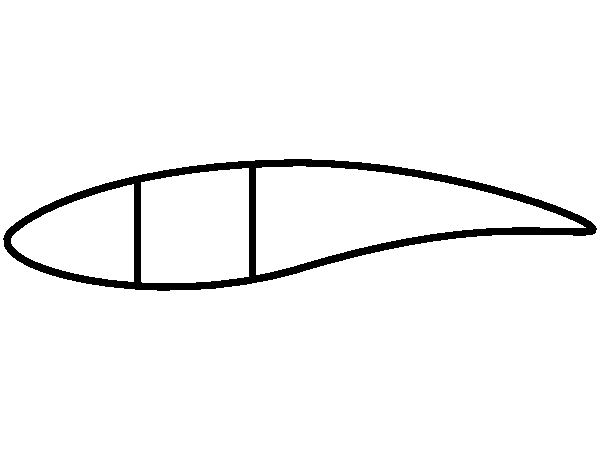
\includegraphics[width=1in]{hollowcore}} &  \parbox[c]{1in}{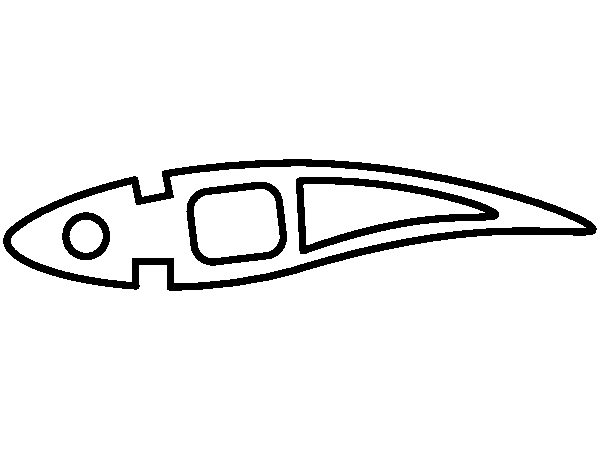
\includegraphics[width=1in]{balsa}} \\
		\hline
		Weight & 10 & & &\\
		\hline
		Strength & 8 & & & \\
		\hline
		Simplicity & 6 & & & \\
		\hline
		Durability & 4 & & & \\
		\hline
		{\color{\BYUred} {\color{BYUred} [YEAR SPECIFIC ITEM]}} & 2 & & & \\
		\hline
		\multicolumn{2}{|c|}{Totals} &  &  &  \\%BOLD WINNING OPTION
		\hline
	\end{tabular}
\end{table}








%----------------
%---   Payload Manufacture Decision Matrix  (single prop, dual prop, distributed propulsion, etc.)
%----------------
\begin{table}[h!]
	\centering
	\caption{Weighted decision matrix for {\color{\BYUred} [SPECIFY THIS YEAR'S PAYLOAD DESIGN]}.}
	\label{tab:payloadmanufacturedecision}
	\rowcolors{2}{BYUbluelite}{white}
	\begin{tabular}{ |c|c|c|c|c| } 
		\hline
		\rowcolor{BYUbluemid}
		& & {\color{BYUred} [OPTION]} & {\color{BYUred} [OPTION]} & {\color{BYUred} [OPTION]} \\
		\rowcolor{BYUbluemid}
		\multirow{-2}{*}{Factor} & \multirow{-2}{*}{Scale}  & \parbox[c]{1in}{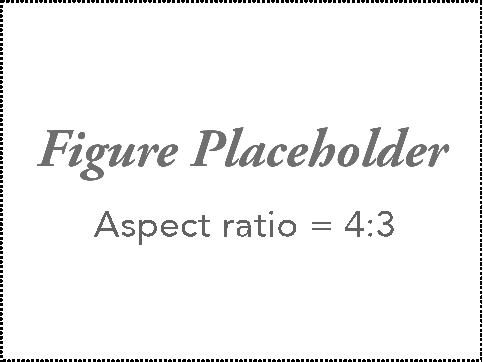
\includegraphics[width=1in]{draft4x3}} & \parbox[c]{1in}{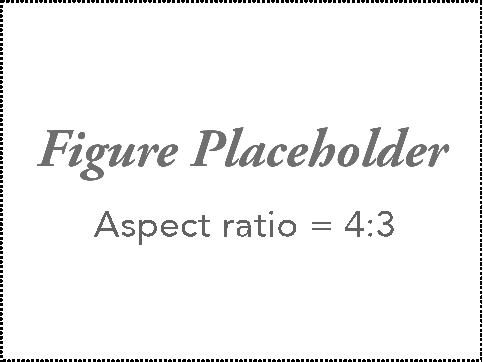
\includegraphics[width=1in]{draft4x3}} &  \parbox[c]{1in}{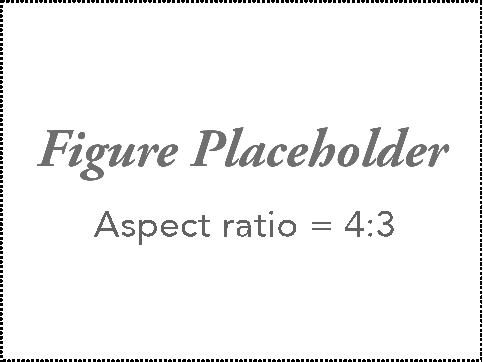
\includegraphics[width=1in]{draft4x3}} \\
		\hline
		Weight & 10 & & &\\
		\hline
		Strength & 8 & & & \\
		\hline
		Simplicity & 6 & & & \\
		\hline
		Durability & 4 & & & \\
		\hline
		{\color{\BYUred} {\color{BYUred} [YEAR SPECIFIC ITEM]}} & 2 & & & \\
		\hline
		\multicolumn{2}{|c|}{Totals} &  &  &  \\%BOLD WINNING OPTION
		\hline
	\end{tabular}
\end{table}

%----------------
% ---  Manufacturing Milestone chart
%----------------
\begin{figure}[h!]
	\centering
	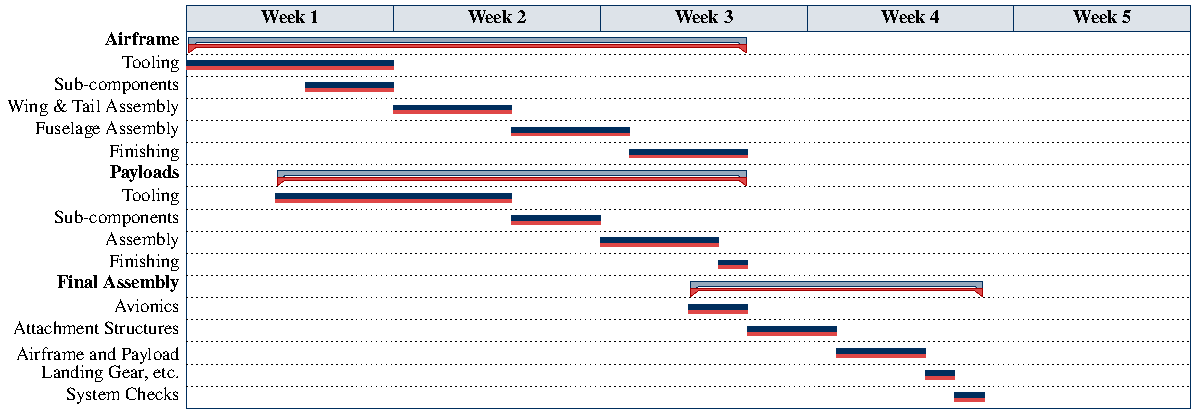
\includegraphics[]{manufacturingchart.pdf}
	\caption{This milestone chart reveals our {\color{\BYUblue}original plan} for major elements of our manufacturing process compared to the {\color{\BYUred}actual timing} of these events for our detailed prototype, we hope to hold to a similar planned schedule for our competition build.}
	\label{fig:plannedvsactualtimingmanufacturing}
\end{figure}



%%%%%%%%%%%%%%%%%%%%%%%%%%%%%%%%%%%%%%%%%%%%%%%%%%%%%%%%%%%%%%%%%%%%%%%%%%%%%%%%%%%%%%%%%
%%%%%%%%%%%%%%%%%%%%%%%%%%%%           TESTING PLAN            %%%%%%%%%%%%%%%%%%%%%%%%%%
%%%%%%%%%%%%%%%%%%%%%%%%%%%%%%%%%%%%%%%%%%%%%%%%%%%%%%%%%%%%%%%%%%%%%%%%%%%%%%%%%%%%%%%%%
\section{Testing Plan} % (5 points)
\label{sec:TestingPlan}
% Section Requirements
% 1) Describe all major ground and flight tests performed.
% 2) Objectives and schedule for each.
% 3) Data to be collected and how applied.
% 4) Test and flight check lists


\subsection{Completed Testing}
\label{ssec:completedtesting}




\paragraph{Ground Testing}
\label{sssec:groundtesting}



\paragraph{Flight Testing}
\label{sssec:flighttesting}



\subsection{Planned Testing}
\label{ssec:plannedtesting}



\subsection{Test and Flight Checklists}



%%%%%%%%%%%%%%%%%%%%%%%%%%%%%%%%%%%%%%%%%%%%%%%%%%%%%%%%%%%%%%%%%%%%%%%%%%%%%%%%%%%%%%%%%
%%%%%%%%%%%%%%%%%%%%%%%%%%          PERFORMANCE RESULTS          %%%%%%%%%%%%%%%%%%%%%%%%
%%%%%%%%%%%%%%%%%%%%%%%%%%%%%%%%%%%%%%%%%%%%%%%%%%%%%%%%%%%%%%%%%%%%%%%%%%%%%%%%%%%%%%%%%
\section{Performance Results} % (10 Points)
\label{sec:PerformanceResults}
% Section Requirements
% ) Describe the demonstrated performance of key subsystems following execution of testing plan
% ) Compare to predictions and explain any differences and improvements made
% ) Describe the demonstrated performance of your complete aircraft solution
% ) Compare to predictions and explain any differences and improvements made






%%%%%%%%%%%%%%%%%%%%%%%%%%%%%%%%%%%%%%%%%%%%%%%%%%%%%%%%%%%%%%%%%%%%%%%%%%%%%%%%%%%%%%%%%
%%%%%%%%%%%%%%%%%%%%%%%%%%%%           BIBLIOGRAPHY            %%%%%%%%%%%%%%%%%%%%%%%%%%
%%%%%%%%%%%%%%%%%%%%%%%%%%%%%%%%%%%%%%%%%%%%%%%%%%%%%%%%%%%%%%%%%%%%%%%%%%%%%%%%%%%%%%%%%
%Bibliography (5 Points)
% 1) List of all published works referenced in the text must be present in this section.
% 2) Any material taken from a published source in all previous sections must have a numerical subscript corresponding to the appropriate citation in this section.
% 3) References should appear in numerical order.
% 4) Format should match AIAA provided guidelines:
%\newpage
%\clearpage
\bibliography{ref}{}
\bibliographystyle{aiaa}

\end{document}